\documentclass[aspectratio=119,12pt]{beamer}

\usepackage{amsmath}
\usepackage{tikz}
\usepackage{pgfplots}
\usepackage{pgfpages}
% \usepackage{svg}

\pgfplotsset{compat=1.18}

\usetheme{default}

\setbeamertemplate{navigation symbols}{}

\pgfpagesuselayout{8 on 1}[
    a4paper,
    border shrink=2mm
]

\setbeamertemplate{background}{
    \begin{tikzpicture}[remember picture,overlay]
        \draw[gray, line width=0.5pt]
            ([xshift=3pt,yshift=-3pt]current page.north west)
            rectangle
            ([xshift=-3pt,yshift=3pt]current page.south east);
    \end{tikzpicture}
}

\begin{document}

%------------------------------------------------
\begin{frame}
    \centering
    \Huge \textbf{Bølger}

    \vspace{1cm}

    \Large
    Hva er en bølge, og hvordan beskriver vi den?
\end{frame}

%------------------------------------------------
\begin{frame}{Hva er en bølge?}

    \begin{center}
        \Large
        En bølge er en svingning som forplanter seg
        og transporterer energi.
    \end{center}

    \vspace{1cm}
    \begin{itemize}
        \item Eksempel: vannbølger, lydbølger, radiobølger, laser
    \end{itemize}
    \vspace{1cm}


    % Er det noen bølger som ikke beveger på seg?
    % \begin{itemize}
    %     \item Eksempel: sykkelvei på ballstad, karusell, et landskap med åser 
    % \end{itemize}



\end{frame}

%------------------------------------------------
\begin{frame}{Hvordan beskriver vi en bølge?}

\begin{center}
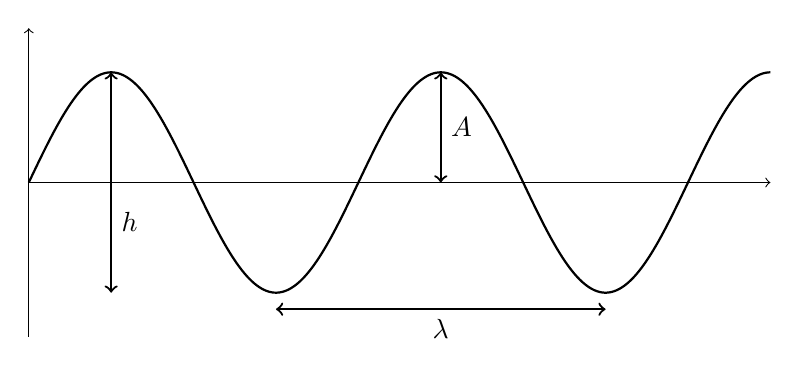
\begin{tikzpicture}
    \begin{axis}[
        width=11cm,
        height=5.5cm,
        axis lines=middle,
        xmin=0, xmax=4.5*pi,
        ymin=-1.4, ymax=1.4,
        xtick=\empty,
        ytick=\empty,
        axis line style={->},
        clip=false
    ]

        % Bølge
        \addplot[
            domain=0:4.5*pi,
            samples=300,
            thick
        ] {sin(deg(x))};

        % Likevektslinje
        \addplot[
            domain=0:4.5*pi,
            dashed
        ] {0};

        % Bølgehøyde
        \draw[<->, thick]
            (axis cs:pi/2,-1)
            -- (axis cs:pi/2,1)
            node[midway,right,yshift=-0.5cm] {$h$};

        % Bølgehøyde
        \draw[<->, thick]
            (axis cs:2*pi + pi/2,0)
            -- (axis cs:2*pi+ pi/2,1)
            node[midway,right,yshift=-0.0cm] {$A$};

        % Bølgelengde
        \draw[<->,thick]
            (axis cs: 3*pi/2 + 0,-1.15)
            -- (axis cs: 3*pi/2 +2*pi,-1.15)
            node[midway,below] {$\lambda$};

    \end{axis}
\end{tikzpicture}
\end{center}


Her definerer vi 
\begin{itemize}
    \item $h$ bølgehøyde er avstanden fra bunnen av bølgen til toppen av bølgen. 
    \item $A$ Amplitude er fra likevekt til toppen av bølgen. Merk $A = \frac{h}{2}$   
    \item $\lambda$ Bølgelengde er avstanden mellom to påfølgende bølgetopper.   

\end{itemize}

\end{frame}


%------------------------------------------------
\begin{frame}{Periode og frekvens}

\Large
\textbf{Periode}

Tiden $T$  det tar for én hel svingning. $[T] = sekund$ 

\vspace{0.5cm}

\textbf{Frekvens}

Hvor mange svingninger som skjer per sekund $f = \frac{1}{T}$. Vi bruker enheten $[f]= \frac{1}{sekund}=\mathrm{Hz}$.


\vspace{0.5cm}

Har vi eksempler på periode og frekvens i den ekte verden? (Mensensyklus, klokke eller årstider)



\end{frame}




%------------------------------------------------
\begin{frame}{Repetisjon: Hastighet}


Finnes det bølger som står i ro eller som beveger seg?  

\begin{center}
\Large

\[
\boxed{v=\frac{s}{t}}
\]

\end{center}

\vspace{0.7cm}

\textbf{Eksempel}

Jacob Ingebrrigsten løp \(400\,\mathrm{m}\) på \(51\,\mathrm{s}\). Da blir gjennsomsnittsfarten

\[
v
=
\frac{400\,\mathrm{m}}{51\,\mathrm{s}}
\approx
7{,}84\,\mathrm{m/s}
\]

\end{frame}



%------------------------------------------------
\begin{frame}{Definisjon av bølgehastighet}

\begin{center}

\Large
\[
\boxed{
v_{\text{bølge}}
=
\frac{\lambda}{T}
}
\]

\end{center}

\vspace{0.7cm}

\textbf{Eksempel}

\[
\lambda=10\,\mathrm{m},
\qquad
T=15\,\mathrm{s}
\]

\[
v_{\text{bølge}}
=
\frac{10\,\mathrm{m}}{15\,\mathrm{s}}
\approx
0{,}67\,\mathrm{m/s}
\]

\[
\approx 2{,}4\,\mathrm{km/t}
\]

\end{frame}

%------------------------------------------------
\begin{frame}{Sammenheng mellom \(v\), \(f\) og \(\lambda\)}

Vi har

\[
v=\frac{\lambda}{T}
\]

og

\[
f=\frac{1}{T}.
\]

Dermed får vi

\[
\boxed{v=f\lambda}
\]

\vspace{0.8cm}

\begin{center}
\Large
\textbf{ bølgefart = frekvens $\times$ bølgelengde}
\end{center}

\end{frame}


\begin{frame}{Animasjon}

\centering
\href{https://isakhammer.github.io/education/index.html}{\texttt{isakhammer.github.io/education}}

\end{frame}


\begin{frame}{Oppsummering}

\[
\boxed{f=\frac{1}{T}}
\]

\[
\boxed{v=\frac{\lambda}{T}}
\]

\[
\boxed{v=f\lambda}
\]

\vspace{0.7cm}

\begin{center}
\Large
Bølgelengde \(\lambda\), periode \(T\), frekvens \(f\)
og hastighet \(v\).
\end{center}

\end{frame}

%------------------------------------------------
\begin{frame}{Spørsmål}

\begin{enumerate}
    \item Hva betyr bølgehøyden \(h\), og hva er forskjellen på det og amplitude? Hvorfor er bølgehøyde et mer nyttig begrep i sjøfart?
    \item Hva er en bølgelengde \(\lambda\)? Kan man måle bølgelengde i en vanlig sjø? Hva med i en radiobølge? 
    \item Hva betyr perioden \(T\)?
    \item Hva er frekvens? Hvorfor er frekvens et nyttig begrep? 
\end{enumerate}

\end{frame}

%------------------------------------------------

\begin{frame}{Eksperiment, hastighet på bølger i fjæra}

    Kan vi med denne informasjonen regne ut hastigheten til bølger i havet?

    \begin{itemize}
        \item Estimer periodetid $T$ . Prøv å ta tiden og hvor mange bølger som slår inn mot land iløpet av 60sek. Da vil du få gjennsomsnittlig periodetid for \textbf{en} bølge.   
        \item Kan vi ca estimere på øyemål hvor lang bølgelengden er? Feks ca 1.0m-1.5m
        \item Bruk formelen $v = \lambda / T  $. Kan dere estimere ca hva er det høyeste estimatet eller det laveste estimatet av hastighet?  
        \item Hvor troverdig er dere på estimatet? kan det stemme? Tror dere at bølgehastigheten er lik når det er dårlig eller fint vær? Hva med fjære versus i dypt vann?   
    \end{itemize}

\end{frame}



\begin{frame}{Elektromagnetiske Spekteret}

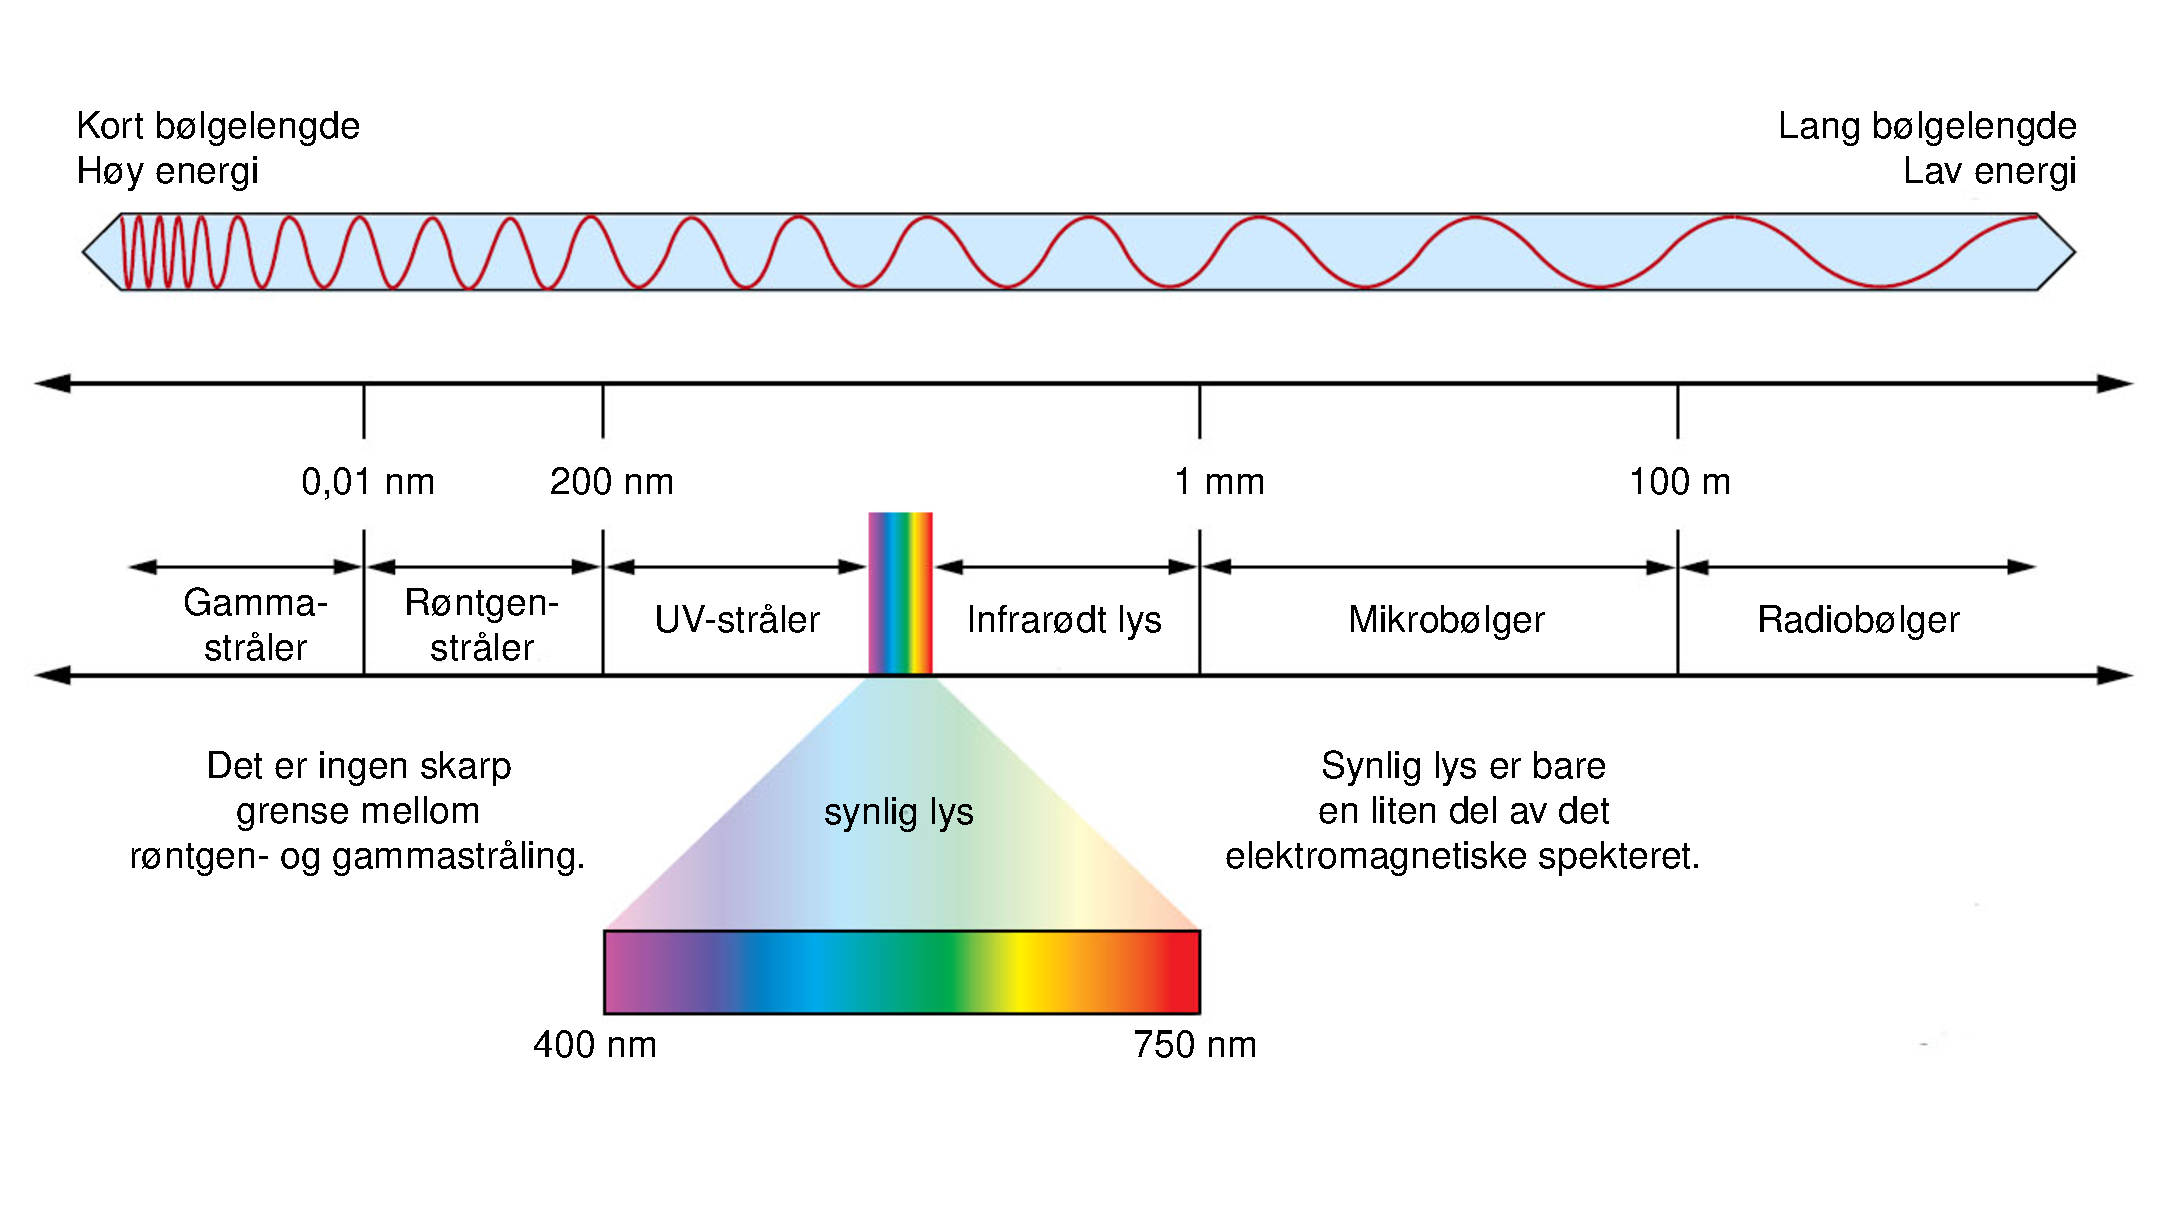
\includegraphics[width=\textwidth]{spekteret.pdf}

\begin{itemize}
    \item Synlig lys er bare en veldig veldig liten del av spekteret.
\item Har dere eksempler på hvilken signaler som blir brukt på hver ende?
\item  Hvilken hastighet har lyset, kan det endre seg? 
\end{itemize}
  

\end{frame}

\begin{frame}{Mikrobølge-ovneksperiement}

    Sammenhengen mellom lysets hastighet $c$, bølgelengden $\lambda$ og frekvensen $f$ er
    \[
        c = f\lambda.
\]
    Dermed kan vi regne ut lysets hastighet dersom vi kjenner bølgelengden og frekvensen.




\end{frame}

\begin{frame}{SI-prefikser}

\begin{table}
\centering
\begin{tabular}{c c c}
\hline
\textbf{Prefiks} & \textbf{Symbol} & \textbf{Faktor} \\
\hline
nano   & n & $10^{-9}$ \\
mikro  & $\mu$ & $10^{-6}$ \\
milli  & m & $10^{-3}$ \\
centi  & c & $10^{-2}$ \\
desi   & d & $10^{-1}$ \\
       &   & $10^0$ \\
kilo   & k & $10^3$ \\
mega   & M & $10^6$ \\
giga   & G & $10^9$ \\
\hline
\end{tabular}
\end{table}

\vspace{0.3cm}

\[
\boxed{
\begin{aligned}
1\,\mathrm{nm}  &= 10^{-9}\,\mathrm{m} \\
1\,\mathrm{ms}  &= 10^{-3}\,\mathrm{s} \\
1\,\mathrm{GHz} &= 10^{9}\,\mathrm{Hz}
\end{aligned}}
\]


\end{frame}






\end{document}
